\documentclass[twoside]{book}

% Packages required by doxygen
\usepackage{fixltx2e}
\usepackage{calc}
\usepackage{doxygen}
\usepackage[export]{adjustbox} % also loads graphicx
\usepackage{graphicx}
\usepackage[utf8]{inputenc}
\usepackage{makeidx}
\usepackage{multicol}
\usepackage{multirow}
\PassOptionsToPackage{warn}{textcomp}
\usepackage{textcomp}
\usepackage[nointegrals]{wasysym}
\usepackage[table]{xcolor}

% Font selection
\usepackage[T1]{fontenc}
\usepackage[scaled=.90]{helvet}
\usepackage{courier}
\usepackage{amssymb}
\usepackage{sectsty}
\renewcommand{\familydefault}{\sfdefault}
\allsectionsfont{%
  \fontseries{bc}\selectfont%
  \color{darkgray}%
}
\renewcommand{\DoxyLabelFont}{%
  \fontseries{bc}\selectfont%
  \color{darkgray}%
}
\newcommand{\+}{\discretionary{\mbox{\scriptsize$\hookleftarrow$}}{}{}}

% Page & text layout
\usepackage{geometry}
\geometry{%
  a4paper,%
  top=2.5cm,%
  bottom=2.5cm,%
  left=2.5cm,%
  right=2.5cm%
}
\tolerance=750
\hfuzz=15pt
\hbadness=750
\setlength{\emergencystretch}{15pt}
\setlength{\parindent}{0cm}
\setlength{\parskip}{0.2cm}
\makeatletter
\renewcommand{\paragraph}{%
  \@startsection{paragraph}{4}{0ex}{-1.0ex}{1.0ex}{%
    \normalfont\normalsize\bfseries\SS@parafont%
  }%
}
\renewcommand{\subparagraph}{%
  \@startsection{subparagraph}{5}{0ex}{-1.0ex}{1.0ex}{%
    \normalfont\normalsize\bfseries\SS@subparafont%
  }%
}
\makeatother

% Headers & footers
\usepackage{fancyhdr}
\pagestyle{fancyplain}
\fancyhead[LE]{\fancyplain{}{\bfseries\thepage}}
\fancyhead[CE]{\fancyplain{}{}}
\fancyhead[RE]{\fancyplain{}{\bfseries\leftmark}}
\fancyhead[LO]{\fancyplain{}{\bfseries\rightmark}}
\fancyhead[CO]{\fancyplain{}{}}
\fancyhead[RO]{\fancyplain{}{\bfseries\thepage}}
\fancyfoot[LE]{\fancyplain{}{}}
\fancyfoot[CE]{\fancyplain{}{}}
\fancyfoot[RE]{\fancyplain{}{\bfseries\scriptsize Generated on Sun Apr 10 2016 23\+:28\+:51 for General Quadratic Placer by Doxygen }}
\fancyfoot[LO]{\fancyplain{}{\bfseries\scriptsize Generated on Sun Apr 10 2016 23\+:28\+:51 for General Quadratic Placer by Doxygen }}
\fancyfoot[CO]{\fancyplain{}{}}
\fancyfoot[RO]{\fancyplain{}{}}
\renewcommand{\footrulewidth}{0.4pt}
\renewcommand{\chaptermark}[1]{%
  \markboth{#1}{}%
}
\renewcommand{\sectionmark}[1]{%
  \markright{\thesection\ #1}%
}

% Indices & bibliography
\usepackage{natbib}
\usepackage[titles]{tocloft}
\setcounter{tocdepth}{3}
\setcounter{secnumdepth}{5}
\makeindex

% Hyperlinks (required, but should be loaded last)
\usepackage{ifpdf}
\ifpdf
  \usepackage[pdftex,pagebackref=true]{hyperref}
\else
  \usepackage[ps2pdf,pagebackref=true]{hyperref}
\fi
\hypersetup{%
  colorlinks=true,%
  linkcolor=blue,%
  citecolor=blue,%
  unicode%
}

% Custom commands
\newcommand{\clearemptydoublepage}{%
  \newpage{\pagestyle{empty}\cleardoublepage}%
}

\usepackage{caption}
\captionsetup{labelsep=space,justification=centering,font={bf},singlelinecheck=off,skip=4pt,position=top}

%===== C O N T E N T S =====

\begin{document}

% Titlepage & ToC
\hypersetup{pageanchor=false,
             bookmarks=true,
             bookmarksnumbered=true,
             pdfencoding=unicode
            }
\pagenumbering{roman}
\begin{titlepage}
\vspace*{7cm}
\begin{center}%
{\Large General Quadratic Placer }\\
\vspace*{1cm}
{\large Generated by Doxygen 1.8.11}\\
\vspace*{0.5cm}
{\small Sun Apr 10 2016 23:28:51}\\
\end{center}
\end{titlepage}
\clearemptydoublepage
\tableofcontents
\clearemptydoublepage
\pagenumbering{arabic}
\hypersetup{pageanchor=true}

%--- Begin generated contents ---
\chapter{Namespace Index}
\section{Packages}
Here are the packages with brief descriptions (if available)\+:\begin{DoxyCompactList}
\item\contentsline{section}{\hyperlink{namespacegqp__placer}{gqp\+\_\+placer} \\*General Quadratic Placer }{\pageref{namespacegqp__placer}}{}
\end{DoxyCompactList}

\chapter{Hierarchical Index}
\section{Class Hierarchy}
This inheritance list is sorted roughly, but not completely, alphabetically\+:\begin{DoxyCompactList}
\item Exception\begin{DoxyCompactList}
\item \contentsline{section}{gqp\+\_\+placer.\+My\+Error}{\pageref{classgqp__placer_1_1MyError}}{}
\end{DoxyCompactList}
\item \contentsline{section}{gqp\+\_\+placer.\+mothercore}{\pageref{classgqp__placer_1_1mothercore}}{}
\end{DoxyCompactList}

\chapter{Class Index}
\section{Class List}
Here are the classes, structs, unions and interfaces with brief descriptions\+:\begin{DoxyCompactList}
\item\contentsline{section}{\hyperlink{classcoo__matrix}{coo\+\_\+matrix} }{\pageref{classcoo__matrix}}{}
\item\contentsline{section}{\hyperlink{classmothercore}{mothercore} }{\pageref{classmothercore}}{}
\end{DoxyCompactList}

\chapter{Namespace Documentation}
\hypertarget{namespacegqp__placer}{}\section{gqp\+\_\+placer Namespace Reference}
\label{namespacegqp__placer}\index{gqp\+\_\+placer@{gqp\+\_\+placer}}


General Quadratic Placer.  


\subsection*{Classes}
\begin{DoxyCompactItemize}
\item 
class \hyperlink{classgqp__placer_1_1mothercore}{mothercore}
\item 
class \hyperlink{classgqp__placer_1_1MyError}{My\+Error}
\end{DoxyCompactItemize}
\subsection*{Functions}
\begin{DoxyCompactItemize}
\item 
def \hyperlink{namespacegqp__placer_a79e959958df02edd23d005c3bd39f76b}{create} (filename)\hypertarget{namespacegqp__placer_a79e959958df02edd23d005c3bd39f76b}{}\label{namespacegqp__placer_a79e959958df02edd23d005c3bd39f76b}

\begin{DoxyCompactList}\small\item\em Creates the \char`\"{}mothercore\char`\"{} class from file. \end{DoxyCompactList}\item 
def \hyperlink{namespacegqp__placer_af9c1a6e7a029032bede284565d4052a0}{solveforx} (core)\hypertarget{namespacegqp__placer_af9c1a6e7a029032bede284565d4052a0}{}\label{namespacegqp__placer_af9c1a6e7a029032bede284565d4052a0}

\begin{DoxyCompactList}\small\item\em Solves the given core for locations of gates. \end{DoxyCompactList}\item 
def \hyperlink{namespacegqp__placer_ac0e10aaeefffce8ac622fa07b37709e6}{writeback} (core, filename)\hypertarget{namespacegqp__placer_ac0e10aaeefffce8ac622fa07b37709e6}{}\label{namespacegqp__placer_ac0e10aaeefffce8ac622fa07b37709e6}

\begin{DoxyCompactList}\small\item\em Read and write back to given filename. \end{DoxyCompactList}\item 
def \hyperlink{namespacegqp__placer_adc1081e9e8526fb4db8748388be1ada5}{assign} (core, G, h\+O\+Rv, l\+O\+Rr)\hypertarget{namespacegqp__placer_adc1081e9e8526fb4db8748388be1ada5}{}\label{namespacegqp__placer_adc1081e9e8526fb4db8748388be1ada5}

\begin{DoxyCompactList}\small\item\em Sorts the gates from the given core according to h\+O\+Rv and l\+O\+Rr 1 horizontal sort, then 1 vertical sort if needed. \end{DoxyCompactList}\item 
def \hyperlink{namespacegqp__placer_a56ef0cdc6c1625b0e9bc0a4ab97d763c}{update\+\_\+coordinates} (coordinate, side)\hypertarget{namespacegqp__placer_a56ef0cdc6c1625b0e9bc0a4ab97d763c}{}\label{namespacegqp__placer_a56ef0cdc6c1625b0e9bc0a4ab97d763c}

\begin{DoxyCompactList}\small\item\em Updates the coordinate according to bounding box. \end{DoxyCompactList}\item 
def \hyperlink{namespacegqp__placer_a600dd4547705a5709ee16989f13591d5}{update\+\_\+location} (core, x, y, key)\hypertarget{namespacegqp__placer_a600dd4547705a5709ee16989f13591d5}{}\label{namespacegqp__placer_a600dd4547705a5709ee16989f13591d5}

\begin{DoxyCompactList}\small\item\em Updates the location values given in the class. \end{DoxyCompactList}\item 
def \hyperlink{namespacegqp__placer_a09d4a51106fd3e91feb0cd3656ea7f4b}{contain\+Nrun} (core, side, h\+O\+Rv, l\+O\+Rr)\hypertarget{namespacegqp__placer_a09d4a51106fd3e91feb0cd3656ea7f4b}{}\label{namespacegqp__placer_a09d4a51106fd3e91feb0cd3656ea7f4b}

\begin{DoxyCompactList}\small\item\em Contains half the gates in core within the bounding box and solves for gate locations. \end{DoxyCompactList}\item 
def \hyperlink{namespacegqp__placer_ab943530c8a95de269a92af84899cb424}{place} (core, side, n)\hypertarget{namespacegqp__placer_ab943530c8a95de269a92af84899cb424}{}\label{namespacegqp__placer_ab943530c8a95de269a92af84899cb424}

\begin{DoxyCompactList}\small\item\em Iterative Placer. \end{DoxyCompactList}\item 
def \hyperlink{namespacegqp__placer_ab87a36d6fec84b4738f9a09178b2d90e}{main} ()\hypertarget{namespacegqp__placer_ab87a36d6fec84b4738f9a09178b2d90e}{}\label{namespacegqp__placer_ab87a36d6fec84b4738f9a09178b2d90e}

\begin{DoxyCompactList}\small\item\em Main. \end{DoxyCompactList}\end{DoxyCompactItemize}


\subsection{Detailed Description}
General Quadratic Placer. 
\chapter{Class Documentation}
\hypertarget{classgqp__placer_1_1mothercore}{}\section{gqp\+\_\+placer.\+mothercore Class Reference}
\label{classgqp__placer_1_1mothercore}\index{gqp\+\_\+placer.\+mothercore@{gqp\+\_\+placer.\+mothercore}}
\subsection*{Public Member Functions}
\begin{DoxyCompactItemize}
\item 
def \hyperlink{classgqp__placer_1_1mothercore_a0fdfdd800f6104a0b6a68599559c750f}{\+\_\+\+\_\+init\+\_\+\+\_\+} (self, \hyperlink{classgqp__placer_1_1mothercore_adda3ce69f8cb37fd8de8fc66e700500a}{side})
\begin{DoxyCompactList}\small\item\em The constructor. \end{DoxyCompactList}\item 
def \hyperlink{classgqp__placer_1_1mothercore_adcbc5a7363bec0ed2557df3b9560c16c}{get\+\_\+numG} (self)
\begin{DoxyCompactList}\small\item\em Helper function to return the number of gates. \end{DoxyCompactList}\item 
def \hyperlink{classgqp__placer_1_1mothercore_ae4aa5a084403ae3fcbedad7fc40b2b0f}{get\+\_\+numP} (self)\hypertarget{classgqp__placer_1_1mothercore_ae4aa5a084403ae3fcbedad7fc40b2b0f}{}\label{classgqp__placer_1_1mothercore_ae4aa5a084403ae3fcbedad7fc40b2b0f}

\begin{DoxyCompactList}\small\item\em Helper function to return the number of pads. \end{DoxyCompactList}\item 
def \hyperlink{classgqp__placer_1_1mothercore_aedecd9639f2d26eb74ebaf94bccd7752}{get\+\_\+numN} (self)\hypertarget{classgqp__placer_1_1mothercore_aedecd9639f2d26eb74ebaf94bccd7752}{}\label{classgqp__placer_1_1mothercore_aedecd9639f2d26eb74ebaf94bccd7752}

\begin{DoxyCompactList}\small\item\em Helper function to return the number of nets. \end{DoxyCompactList}\item 
def \hyperlink{classgqp__placer_1_1mothercore_a2b73ac270372e97d8e990effedd75d17}{set\+\_\+side} (self, \hyperlink{classgqp__placer_1_1mothercore_adda3ce69f8cb37fd8de8fc66e700500a}{side})\hypertarget{classgqp__placer_1_1mothercore_a2b73ac270372e97d8e990effedd75d17}{}\label{classgqp__placer_1_1mothercore_a2b73ac270372e97d8e990effedd75d17}

\begin{DoxyCompactList}\small\item\em Helper function to set the side variable. \end{DoxyCompactList}\item 
def \hyperlink{classgqp__placer_1_1mothercore_a9d4ec1ac49ac17f5d4ce7c4c743cbc96}{get\+\_\+gate} (self)\hypertarget{classgqp__placer_1_1mothercore_a9d4ec1ac49ac17f5d4ce7c4c743cbc96}{}\label{classgqp__placer_1_1mothercore_a9d4ec1ac49ac17f5d4ce7c4c743cbc96}

\begin{DoxyCompactList}\small\item\em Helper function to return a dictionary of gates. \end{DoxyCompactList}\item 
def \hyperlink{classgqp__placer_1_1mothercore_a396e123fe8d6cbad16f828dd21c56132}{get\+\_\+gateconnections} (self, gatenum)\hypertarget{classgqp__placer_1_1mothercore_a396e123fe8d6cbad16f828dd21c56132}{}\label{classgqp__placer_1_1mothercore_a396e123fe8d6cbad16f828dd21c56132}

\begin{DoxyCompactList}\small\item\em Helper function which returns the connections of given gate. \end{DoxyCompactList}\item 
def {\bfseries get\+\_\+gatelocation} (self, gatenum)\hypertarget{classgqp__placer_1_1mothercore_a5fc0b24a700a395afd65bb703f887e41}{}\label{classgqp__placer_1_1mothercore_a5fc0b24a700a395afd65bb703f887e41}

\item 
def {\bfseries get\+\_\+pad} (self)\hypertarget{classgqp__placer_1_1mothercore_a4729070c9a33e5e87a0c2cae03775e67}{}\label{classgqp__placer_1_1mothercore_a4729070c9a33e5e87a0c2cae03775e67}

\item 
def {\bfseries get\+\_\+padlocation} (self, padnum)\hypertarget{classgqp__placer_1_1mothercore_ad3d0a4a7e7c542864c4ba2adcfd7280a}{}\label{classgqp__placer_1_1mothercore_ad3d0a4a7e7c542864c4ba2adcfd7280a}

\item 
def {\bfseries add\+\_\+gate} (self, gatenum, listofconnections)\hypertarget{classgqp__placer_1_1mothercore_a179455b7cde50fb0c8ff3dd35be55ca1}{}\label{classgqp__placer_1_1mothercore_a179455b7cde50fb0c8ff3dd35be55ca1}

\item 
def {\bfseries add\+\_\+pad} (self, padnum, netandlocation)\hypertarget{classgqp__placer_1_1mothercore_aa4899f06601a4a1e19b3e5bce4f99bfc}{}\label{classgqp__placer_1_1mothercore_aa4899f06601a4a1e19b3e5bce4f99bfc}

\item 
def {\bfseries add\+\_\+net} (self, netnum, connection, gateorpad)\hypertarget{classgqp__placer_1_1mothercore_a0bcf31558757a0edd15a586468715378}{}\label{classgqp__placer_1_1mothercore_a0bcf31558757a0edd15a586468715378}

\item 
def {\bfseries add\+\_\+netconns} (self, netnum, listofconnections)\hypertarget{classgqp__placer_1_1mothercore_aff93e1055cd53093faf6ec7e743f8433}{}\label{classgqp__placer_1_1mothercore_aff93e1055cd53093faf6ec7e743f8433}

\item 
def {\bfseries get\+\_\+otherconns} (self, netnum, gatenum)\hypertarget{classgqp__placer_1_1mothercore_a8ca67285ee77dac596b73128c9b655af}{}\label{classgqp__placer_1_1mothercore_a8ca67285ee77dac596b73128c9b655af}

\item 
def {\bfseries get\+\_\+nets} (self)\hypertarget{classgqp__placer_1_1mothercore_aeea04940559af5cbcf30f508d6d89d19}{}\label{classgqp__placer_1_1mothercore_aeea04940559af5cbcf30f508d6d89d19}

\item 
def {\bfseries add\+\_\+location} (self, x, y, data)\hypertarget{classgqp__placer_1_1mothercore_a241bd6a3a70001d27965250630df7558}{}\label{classgqp__placer_1_1mothercore_a241bd6a3a70001d27965250630df7558}

\item 
def \hyperlink{classgqp__placer_1_1mothercore_a66c7983b80befa6e904a94e3e0621335}{add\+\_\+sorted} (self, sort)\hypertarget{classgqp__placer_1_1mothercore_a66c7983b80befa6e904a94e3e0621335}{}\label{classgqp__placer_1_1mothercore_a66c7983b80befa6e904a94e3e0621335}

\begin{DoxyCompactList}\small\item\em Helper function to add a sorted list of gates. \end{DoxyCompactList}\item 
def {\bfseries get\+\_\+sorted} (self)\hypertarget{classgqp__placer_1_1mothercore_a0b7370acc65d6940cc5e200bb53cae1e}{}\label{classgqp__placer_1_1mothercore_a0b7370acc65d6940cc5e200bb53cae1e}

\item 
def {\bfseries get\+\_\+location} (self)\hypertarget{classgqp__placer_1_1mothercore_ae1782ee57912d541a5ea81111eb68db6}{}\label{classgqp__placer_1_1mothercore_ae1782ee57912d541a5ea81111eb68db6}

\end{DoxyCompactItemize}
\subsection*{Public Attributes}
\begin{DoxyCompactItemize}
\item 
\hyperlink{classgqp__placer_1_1mothercore_a31b9c9d21558f6f7b1b18503dd6523d3}{gate}\hypertarget{classgqp__placer_1_1mothercore_a31b9c9d21558f6f7b1b18503dd6523d3}{}\label{classgqp__placer_1_1mothercore_a31b9c9d21558f6f7b1b18503dd6523d3}

\begin{DoxyCompactList}\small\item\em Dictionary of gates. \end{DoxyCompactList}\item 
\hyperlink{classgqp__placer_1_1mothercore_a81bb175f792b80a14b5b67eff710667c}{pad}\hypertarget{classgqp__placer_1_1mothercore_a81bb175f792b80a14b5b67eff710667c}{}\label{classgqp__placer_1_1mothercore_a81bb175f792b80a14b5b67eff710667c}

\begin{DoxyCompactList}\small\item\em Dictionary of pads. \end{DoxyCompactList}\item 
\hyperlink{classgqp__placer_1_1mothercore_a76218cb64486a2f8e243d152812a7fb8}{numG}\hypertarget{classgqp__placer_1_1mothercore_a76218cb64486a2f8e243d152812a7fb8}{}\label{classgqp__placer_1_1mothercore_a76218cb64486a2f8e243d152812a7fb8}

\begin{DoxyCompactList}\small\item\em Number of gates. \end{DoxyCompactList}\item 
\hyperlink{classgqp__placer_1_1mothercore_a8431351d2658faca420f7608bb53bcb1}{numP}\hypertarget{classgqp__placer_1_1mothercore_a8431351d2658faca420f7608bb53bcb1}{}\label{classgqp__placer_1_1mothercore_a8431351d2658faca420f7608bb53bcb1}

\begin{DoxyCompactList}\small\item\em Number of pads. \end{DoxyCompactList}\item 
\hyperlink{classgqp__placer_1_1mothercore_a3e60a21248746eb595abb975dc8d7589}{numN}\hypertarget{classgqp__placer_1_1mothercore_a3e60a21248746eb595abb975dc8d7589}{}\label{classgqp__placer_1_1mothercore_a3e60a21248746eb595abb975dc8d7589}

\begin{DoxyCompactList}\small\item\em Number of nets. \end{DoxyCompactList}\item 
\hyperlink{classgqp__placer_1_1mothercore_adda3ce69f8cb37fd8de8fc66e700500a}{side}\hypertarget{classgqp__placer_1_1mothercore_adda3ce69f8cb37fd8de8fc66e700500a}{}\label{classgqp__placer_1_1mothercore_adda3ce69f8cb37fd8de8fc66e700500a}

\begin{DoxyCompactList}\small\item\em List of 4 elements storing grid limits \mbox{[}xmin, xmax, ymin, ymax\mbox{]}. \end{DoxyCompactList}\item 
\hyperlink{classgqp__placer_1_1mothercore_aafb11667ac74ea67fe71d51e3eca50af}{gateX}\hypertarget{classgqp__placer_1_1mothercore_aafb11667ac74ea67fe71d51e3eca50af}{}\label{classgqp__placer_1_1mothercore_aafb11667ac74ea67fe71d51e3eca50af}

\begin{DoxyCompactList}\small\item\em Dictionary of X coordinates. \end{DoxyCompactList}\item 
\hyperlink{classgqp__placer_1_1mothercore_a56d4174c727a7daf21e8bd9a609e4d11}{gateY}\hypertarget{classgqp__placer_1_1mothercore_a56d4174c727a7daf21e8bd9a609e4d11}{}\label{classgqp__placer_1_1mothercore_a56d4174c727a7daf21e8bd9a609e4d11}

\begin{DoxyCompactList}\small\item\em Dictionary of Y coordinates. \end{DoxyCompactList}\item 
\hyperlink{classgqp__placer_1_1mothercore_a634ce0bcaab7bdc0bb511017a2d698dc}{nets}\hypertarget{classgqp__placer_1_1mothercore_a634ce0bcaab7bdc0bb511017a2d698dc}{}\label{classgqp__placer_1_1mothercore_a634ce0bcaab7bdc0bb511017a2d698dc}

\begin{DoxyCompactList}\small\item\em Dictionary of nets. \end{DoxyCompactList}\item 
\hyperlink{classgqp__placer_1_1mothercore_aca66cf3901dd7c704fffc88e8972391c}{sortedgate}\hypertarget{classgqp__placer_1_1mothercore_aca66cf3901dd7c704fffc88e8972391c}{}\label{classgqp__placer_1_1mothercore_aca66cf3901dd7c704fffc88e8972391c}

\begin{DoxyCompactList}\small\item\em List of sorted gates. \end{DoxyCompactList}\end{DoxyCompactItemize}


\subsection{Constructor \& Destructor Documentation}
\index{gqp\+\_\+placer\+::mothercore@{gqp\+\_\+placer\+::mothercore}!\+\_\+\+\_\+init\+\_\+\+\_\+@{\+\_\+\+\_\+init\+\_\+\+\_\+}}
\index{\+\_\+\+\_\+init\+\_\+\+\_\+@{\+\_\+\+\_\+init\+\_\+\+\_\+}!gqp\+\_\+placer\+::mothercore@{gqp\+\_\+placer\+::mothercore}}
\subsubsection[{\+\_\+\+\_\+init\+\_\+\+\_\+(self, side)}]{\setlength{\rightskip}{0pt plus 5cm}def gqp\+\_\+placer.\+mothercore.\+\_\+\+\_\+init\+\_\+\+\_\+ (
\begin{DoxyParamCaption}
\item[{}]{self, }
\item[{}]{side}
\end{DoxyParamCaption}
)}\hypertarget{classgqp__placer_1_1mothercore_a0fdfdd800f6104a0b6a68599559c750f}{}\label{classgqp__placer_1_1mothercore_a0fdfdd800f6104a0b6a68599559c750f}


The constructor. 



\subsection{Member Function Documentation}
\index{gqp\+\_\+placer\+::mothercore@{gqp\+\_\+placer\+::mothercore}!get\+\_\+numG@{get\+\_\+numG}}
\index{get\+\_\+numG@{get\+\_\+numG}!gqp\+\_\+placer\+::mothercore@{gqp\+\_\+placer\+::mothercore}}
\subsubsection[{get\+\_\+num\+G(self)}]{\setlength{\rightskip}{0pt plus 5cm}def gqp\+\_\+placer.\+mothercore.\+get\+\_\+numG (
\begin{DoxyParamCaption}
\item[{}]{self}
\end{DoxyParamCaption}
)}\hypertarget{classgqp__placer_1_1mothercore_adcbc5a7363bec0ed2557df3b9560c16c}{}\label{classgqp__placer_1_1mothercore_adcbc5a7363bec0ed2557df3b9560c16c}


Helper function to return the number of gates. 



The documentation for this class was generated from the following file\+:\begin{DoxyCompactItemize}
\item 
gqp\+\_\+placer.\+py\end{DoxyCompactItemize}

\hypertarget{classgqp__placer_1_1MyError}{}\section{gqp\+\_\+placer.\+My\+Error Class Reference}
\label{classgqp__placer_1_1MyError}\index{gqp\+\_\+placer.\+My\+Error@{gqp\+\_\+placer.\+My\+Error}}
Inheritance diagram for gqp\+\_\+placer.\+My\+Error\+:\begin{figure}[H]
\begin{center}
\leavevmode
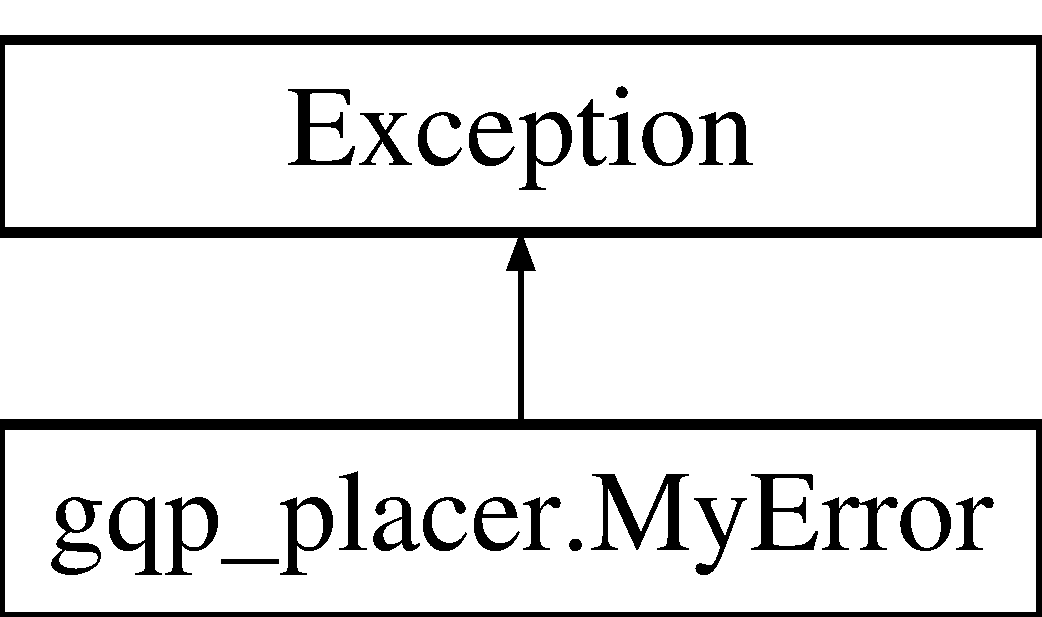
\includegraphics[height=2.000000cm]{classgqp__placer_1_1MyError}
\end{center}
\end{figure}
\subsection*{Public Member Functions}
\begin{DoxyCompactItemize}
\item 
def \hyperlink{classgqp__placer_1_1MyError_a204fcae8bf83a073249c9fcd36846ce6}{\+\_\+\+\_\+init\+\_\+\+\_\+} (self, value)
\begin{DoxyCompactList}\small\item\em The constructor. \end{DoxyCompactList}\end{DoxyCompactItemize}
\subsection*{Public Attributes}
\begin{DoxyCompactItemize}
\item 
{\bfseries value}\hypertarget{classgqp__placer_1_1MyError_a7d623a25feb21771fd937aad5882bd4f}{}\label{classgqp__placer_1_1MyError_a7d623a25feb21771fd937aad5882bd4f}

\end{DoxyCompactItemize}


\subsection{Constructor \& Destructor Documentation}
\index{gqp\+\_\+placer\+::\+My\+Error@{gqp\+\_\+placer\+::\+My\+Error}!\+\_\+\+\_\+init\+\_\+\+\_\+@{\+\_\+\+\_\+init\+\_\+\+\_\+}}
\index{\+\_\+\+\_\+init\+\_\+\+\_\+@{\+\_\+\+\_\+init\+\_\+\+\_\+}!gqp\+\_\+placer\+::\+My\+Error@{gqp\+\_\+placer\+::\+My\+Error}}
\subsubsection[{\+\_\+\+\_\+init\+\_\+\+\_\+(self, value)}]{\setlength{\rightskip}{0pt plus 5cm}def gqp\+\_\+placer.\+My\+Error.\+\_\+\+\_\+init\+\_\+\+\_\+ (
\begin{DoxyParamCaption}
\item[{}]{self, }
\item[{}]{value}
\end{DoxyParamCaption}
)}\hypertarget{classgqp__placer_1_1MyError_a204fcae8bf83a073249c9fcd36846ce6}{}\label{classgqp__placer_1_1MyError_a204fcae8bf83a073249c9fcd36846ce6}


The constructor. 



The documentation for this class was generated from the following file\+:\begin{DoxyCompactItemize}
\item 
gqp\+\_\+placer.\+py\end{DoxyCompactItemize}

%--- End generated contents ---

% Index
\backmatter
\newpage
\phantomsection
\clearemptydoublepage
\addcontentsline{toc}{chapter}{Index}
\printindex

\end{document}
